% !TEX root = main.tex
In this section, we show how to compute an upper bound on $\rho$, with a user-defined confidence $\beta \in (0, 1)$. We do this by constructing a $l$-step CQLF which is valid with probability at least $\beta$. Note that, the existence of a $l$-step CQLF implies $\rho \leq 1$ due to Theorem \ref{thm:cqlf}.

In Section~\ref{sec:stab}, we have given an optimization problem, \eqref{eqn:campiOpt2}, that provides a stability guarantee. Nevertheless, solving this problem as stated is not possible since it involves infinitely many constraints. We consider then the following optimization problem:
\begin{equation}\label{eq:lowerbound}
\begin{aligned}
& \text{min}_P & & \gamma \\
& \text{s.t.} 
&  & (A_{j_l} A_{j_{l-1}} \dots A_{j_1} x)^T P (A_{j_l} A_{j_{l-1}} \dots A_{j_1} x) \leq \gamma^{2l} x^T P x \  \forall\ (x, j_1,\dots, j_l) \in \omega_N\\
& && P \succ 0,\ \gamma \geq 0. \\
\end{aligned}
\end{equation}

Note that, \eqref{eq:lowerbound} can be efficiently solved by semidefinite programming and bisection on the variable $\gamma$ (see \cite{boyd}). Let us denote from now by $\gamma^*(\omega_N)$ the optimal solution of this problem, which we will use to compute a (probabilistic) upper bound on the JSR.





%In this section, we show how to compute an upper bound on $\rho$, with a user-defined confidence $\beta \in (0, 1)$. We do this by constructing a\rmj{n $l$-step CQLF} which is valid with probability at least $\beta$. Note that, the existence of a\rmj{n $l$-step CQLF} implies $\rho \leq 1$ due to Theorem \ref{thm:cqlf}.

%Therefore, to obtain an upper bound on $\rho$, we consider the following optimization problem:
%\begin{equation}\label{eqn:campiOpt0}
%\begin{aligned}
%& \text{min}_{\gamma, P} & & \gamma \\
%& \text{s.t.} 
%&  & (Ax)^TP(Ax) \leq \gamma^2 x^TPx,\,\forall A \in \calM, \,\forall\, x \in \sphere,\\
%& && P \succ 0. \\
%\end{aligned}
%\end{equation}
%Note that, for all $A \in \calM$ the optimal $P$ and the optimal $\gamma$ for the Problem \eqref{eqn:campiOpt0} satisfies: $\frac{A}{\gamma}^TP\frac{A}{\gamma} \preceq P$. Therefore, $\rho\left(\frac{\calM}{\gamma}\right) \leq 1$, which leads to the upper bound $\rho\left(\calM \right) \leq \gamma$.

% Therefore, we instead sample $N$ initial states and modes uniformly random from the set $Z :=\sphere \times M$, and solve the following optimization problem with finitely many constraints instead:
%\begin{equation}\label{eqn:campiOpt00}
%\begin{aligned}
%& \text{min}_{\gamma, P} & & \gamma \\
%& \text{s.t.} 
%&  & (Ax)^TP(Ax) \leq \gamma^2 x^TPx,\,\forall (x, j) \in \omega_N,\\
%& && P \succ 0. \\
%\end{aligned}
%\end{equation}
%where $\omega_N$ is a $N$-uniform random sampling of the set \mbox{$Z:=\sphere \times M$}.
%Note that, since \eqref{eqn:campiOpt00} is convex for a fixed $\gamma$, we can perform bisection on $\gamma$ and solve a series of feasibility problems in $P$ instead. 
Let us analyze the relationship between the solutions of the theoretical optimization problem \eqref{eqn:campiOpt2} and the practical version \eqref{eq:lowerbound}, with finitely many constraints. Even though in practice, one would solve the optimization problem  \eqref{eq:lowerbound} as suggested above, for the sake of rigor and clarity of our proofs, we introduce a slighly different optimization problem. In this new optimization problem, an objective function is considered, and a ``regularization parameter'', $\eta > 0$, is added. As the reader will see, we will derive results valid for arbitrarily small values of $\eta$, and so this will not hamper the practical accuracy of our technique, while allowing us to derive a theoretical asymptotic guarantee (i.e. for large number of observations).

\begin{equation}\label{eqn:campiOpt03}
\begin{aligned}
& \text{min}_{P} & & \lambda_{\max}(P) \\
& \text{s.t.} 
&  & (A_{j_l} A_{j_{l-1}} \dots A_{j_1} x)^T P (A_{j_l} A_{j_{l-1}} \dots A_{j_1} x) \leq {((1 +\eta)\gamma^*(\omega_N))}^{2l} x^T P x,\\
&&&\qquad \qquad \qquad \qquad \quad \qquad \forall (x, j_{1},\dots, j_{l}) \in \omega_N \subset Z_l \\
& && P \succeq I, \\
\end{aligned}
\end{equation}
where $Z_l:= \sphere \times M^l$, $\eta > 0$, and $\gamma^*(\omega_N)$ is the optimal solution to the optimization problem \eqref{eq:lowerbound}. Recall that $\omega_N$ is a given uniform random sample on the set $Z_l$ and of size $N$. 

For the rest of the discussion, we refer to the optimization problem \eqref{eqn:campiOpt03} by $ \Opt(\omega_N)$. We denote its optimal solution by $P(\omega_N)$. We drop the explicit dependence of $P$ on $\omega_N$ when it is clear from the context. There are a few points that are worth noting about \eqref{eqn:campiOpt03}. Firstly, due to Property \ref{property:homogeneity}, we can replace the constraint $P \succ 0$ with the constraint $P \succeq I$. Moreover, for reasons that will become clear later in the discussion, we chose the objective function as $\lambda_{\max}(P)$, instead of solving a feasibility problem in $P$. Lastly, the additional $\eta$ factor is introduced to ensure strict feasibility of \eqref{eqn:campiOpt03}, which will be helpful in the following discussion.

The curious question whether the optimal solution of the sampled problem $\Opt(\omega_N)$ is a feasible solution to \eqref{eqn:campiOpt1} has been widely studied in the literature \cite{campi}. It turns out that under certain technical assumptions, one can bound the proportion of the constraints of the original problem \eqref{eqn:campiOpt1} that are violated by the optimal solution of \eqref{eqn:campiOpt02}, with some probability which is a function of the sample size $N$. 

%\begin{definition}(from \cite{campi}) Consider the optimization problem $\Opt(\omega_N)$ where the set of constraints $\omega_N$ is randomly sampled according to a measure $\mu$. We define the \emph{constraint violation probability} as:
%\begin{equation}\label{eqn:violation0}
%\calV^*(\omega_N)=
%      \mu\left(z \in Z: f(P(\omega_N), z) > 0\right).
%\end{equation}
%Note that, since we have $\mathbb{P}(\calA) = \frac{\mu(\calA)}{\mu(Z)}$, we can rewrite \eqref{eqn:violation0} as:
%\begin{equation*}
%\calV^*(\omega_N)=
%      \frac{\mu(V(\omega_N))}{\mu(Z)},
%\end{equation*}
%where $V(\omega_N):=\{z \in Z: f(P(\omega_N), z) > 0\},$ i.e., the set of points for which at least one constraint is violated for the sampling $\omega_N$.
%\end{definition}
%
%The following theorem from \cite{campi} gives an explicit relationship between $\calV^*(\omega_N)$, $N$, and $n$.
%\begin{theorem}\label{thm:campi}Let $d:=\frac{n(n+1)}{2}+1$ and $N \geq d+1$. Consider the optimization problem $\Opt(\omega_N)$ given in \eqref{eqn:campiOpt01}. If $\Opt(\omega_N)$ satisfies the following technical assumptions:
%\begin{enumerate}
%\item When the problem $\Opt(\omega_N)$ admits an optimal solution, this solution is unique.
%\item Problem $\Opt(\omega_N)$ is nondegenerate\footnote{\textcolor{red}{Explain this in a footnote maybe?}} with probability one.
%\end{enumerate}
%Then, for all $\epsilon \in (0,1)$ the following holds:
%\begin{equation*}\mathbb{P}^N\{\calV^*(\omega_N) \leq \epsilon \} \geq 1- \sum_{j=0}^{d} \binom{N}{j}\epsilon^j (1-\epsilon)^{N-j}.\end{equation*}
%\end{theorem}
%Note that, $\epsilon$ is a constant can be interpreted as the ratio of the measure of points in $Z$ that might violate at least one of the constraints in \eqref{eqn:campiOpt01} to the measure of all points in $Z$.
In the following theorem, we adapt a classical result from random convex optimization literature to our problem.



\begin{theorem}[adapted from Theorem 3.3\footnotemark, \cite{campi}]\label{mainTheorem0}
Let $d$ be the dimension of $\Opt(\omega_N)$ and $N \geq d+1$. Consider the optimization problem $\Opt(\omega_N)$ given in \eqref{eqn:campiOpt02}, where $\omega_N$ is a uniform random sample drawn from the set $Z_l$.
Then, for all $\epsilon \in (0,1)$ the following holds:
\begin{equation}\label{eqn:violation}
\mu_l^N\hspace{-1mm}\left\{ \omega_N \in Z_l^N: \mu_l(V(\omega_N)) \leq \epsilon \right\}\hspace{-1mm} \geq 1- \sum_{j=0}^{d} \binom{N}{j}\epsilon^j (1-\epsilon)^{N-j},\end{equation}
where $\mu_l^N$ denotes the product probability measure on $Z_l^N$, and $V(\omega_N)$ is defined by 
$$V(\omega_N) := \{z=(x,j_{1},\dots,j_{l}) \in Z_l: (A_{j_l} A_{j_{l-1}} \dots A_{j_1} x)^T P(\omega_N)(A_{j_l} A_{j_{l-1}} \dots A_{j_1} x) > (\gamma_{\omega_N}^{*})^{2l} x^T P(\omega_N) x\},$$
i.e., it is the set of constraints that are violated by the optimal solution of $\Opt(\omega_N)$.
\end{theorem}

\footnotetext{Theorem 3.3 in \cite{campi} requires $\Opt(\omega_N)$ to satisfy the following technical assumptions:
\begin{enumerate}
\item When the problem $\Opt(\omega_N)$ admits an optimal solution, this solution is unique.
\item Problem $\Opt(\omega_N)$ is nondegenerate with probability $1$.
\end{enumerate}
Here, the first assumption can be enforced if required by adding a tie-breaking rule to $\Opt(\omega_N)$ as explained in Appendix A in \cite{tiebreak}, while the second assumption can be lifted, as explained in PART 2b in \cite{nondegen}, thanks to the introduction of a ``constraint heating''.
}

%Note that, the assumptions given in the statement of the theorem are of technical nature. That is, if any of the two does not hold for the optimization problem $\Opt(\omega_N)$, it is possible to construct a slightly modified optimization problem for which they indeed hold and work with this modified optimization problem instead. We refer the interested reader to \cite{campi} for a more detailed discussion of such modification techniques.

%\begin{proof}Note that the optimization problem $\Opt(\omega_N)$
%can be written as:
%\begin{equation}
%\label{eqn:campiOpt2}
%\begin{aligned}
%& \text{min}_{P, t} & & t \\
%& \text{s.t.} 
%& & g_{\gamma^*}(P,t,z) \leq 0,\,\forall\ z \in Z\end{aligned}
%\end{equation}
%where $g_{\gamma^*}(P,t,z) = \max(g_1(P, z), g_2(P), g_3(P, t))$, and 
%\begin{eqnarray*}
%g_1(P, z) &=& (A_j z)^TP(A_j z) - {\gamma^*}^2 z^TPz \\
%g_2(P) &=& \lambda_{\max}(-P) +1. \\
%g_3(P,t) &=&  \lambda_{\max}(P) - t.
%\end{eqnarray*}
%The objective function of \eqref{eqn:campiOpt2} is linear while each constraint is convex in $P$ for all $z \in Z$. Also note that, the set of decision variables is in $\R^{\frac{n(n+1)}{2}+1}.$  Then, we can invoke Theorem 3.3 in \cite{campi} with the optimization problem \eqref{eqn:campiOpt2} to conclude the statement of the theorem, with $d=\frac{n(n+1)}{2}+1.$
%\end{proof}

%Theorem \ref{mainTheorem0} states that the optimal solution of the sampled problem $\Opt(\omega_N)$ violates no more than an $\epsilon$ fraction of the constraints in the original optimization problem  \eqref{eqn:campiOpt2} with probability $\beta$, where $\beta$ goes to $1$ as $N$ goes to infinity. This means that, the ellipsoid computed by $\Opt(\omega_N)$ is ``almost invariant"  except on a set of measure $\epsilon$. The rest of this section builds on this, and it has two important intermediate results leading us to our main theorem. 


The above theorem allows us to conclude, from a finite number of observations, that with probability $\beta$ (where $\beta$ goes to $1$ as $N$ goes to infinity), the required property is actually satisfied for the complete sphere $\sphere$, except on a small set of measure at most $\epsilon$. This means that, the ellipsoid computed by $\Opt(\omega_N)$ is ``almost invariant"  except on a set of measure bounded by $\epsilon$. This can be representend in the case $n=2$ by the following plot, where the points of the ellipse in red are points that might violate the contractivity constraint (the set of red points has measure at most $\epsilon$).


\begin{center}
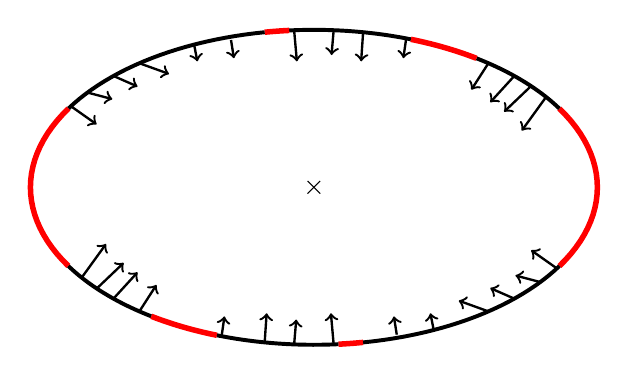
\begin{tikzpicture}[scale=0.8]
\draw (-0.1,-0.1) -- (0.1,0.1);
\draw (-0.1,0.1) -- (0.1,-0.1);
\draw [line width = 0.7mm,red,domain=-30:30] plot ({4.5 * cos(\x)}, {2.5 * sin(\x)});
\draw [line width = 0.5mm,black,domain=30:55] plot ({4.5 * cos(\x)}, {2.5 * sin(\x)});
\draw [line width = 0.7mm,red,domain=55:70] plot ({4.5 * cos(\x)}, {2.5 * sin(\x)});
\draw [line width = 0.5mm,black,domain=70:95] plot ({4.5 * cos(\x)}, {2.5 * sin(\x)});
\draw [line width = 0.7mm,red,domain=95:100] plot ({4.5 * cos(\x)}, {2.5 * sin(\x)});
\draw [line width = 0.5mm,black,domain=100:150] plot ({4.5 * cos(\x)}, {2.5 * sin(\x)});
\draw [line width = 0.7mm,red,domain=150:210] plot ({4.5 * cos(\x)}, {2.5 * sin(\x)});
\draw [line width = 0.5mm,black,domain=210:235] plot ({4.5 * cos(\x)}, {2.5 * sin(\x)});
\draw [line width = 0.7mm,red,domain=235:250] plot ({4.5 * cos(\x)}, {2.5 * sin(\x)});
\draw [line width = 0.5mm,black,domain=250:275] plot ({4.5 * cos(\x)}, {2.5 * sin(\x)});
\draw [line width = 0.7mm,red,domain=275:280] plot ({4.5 * cos(\x)}, {2.5 * sin(\x)});
\draw [line width = 0.5mm,black,domain=280:330] plot ({4.5 * cos(\x)}, {2.5 * sin(\x)});
\draw[->,line width = 0.3mm] (3.6862,1.4339) -- (3.3,0.9);
\draw[->,line width = 0.3mm] (3.4472,1.6070) -- (3.02,1.2);
\draw[->,line width = 0.3mm] (3.182,1.7678) -- (2.8,1.35);
\draw[->,line width = 0.3mm] (2.7705,1.97) -- (2.5,1.55);
\draw[->,line width = 0.3mm] (-3.6862,-1.4339) -- (-3.3,-0.9);
\draw[->,line width = 0.3mm] (-3.4472,-1.6070) -- (-3.02,-1.2);
\draw[->,line width = 0.3mm] (-3.182,-1.7678) -- (-2.8,-1.35);
\draw[->,line width = 0.3mm] (-2.7705,-1.97) -- (-2.5,-1.55);
\draw[->,line width = 0.3mm] (1.4651,2.3638) -- (1.42,2.05);
\draw[->,line width = 0.3mm] (0.7814,2.4620) -- (0.75,2);
\draw[->,line width = 0.3mm] (0.3139,2.4939) -- (0.28,2.1);
\draw[->,line width = 0.3mm] (-0.3139,2.4939) -- (-0.27,2);      
\draw[->,line width = 0.3mm] (-1.4651,-2.3638) -- (-1.42,-2.05);
\draw[->,line width = 0.3mm] (-0.7814,-2.4620) -- (-0.75,-2);
\draw[->,line width = 0.3mm] (-0.3139,-2.4939) -- (-0.28,-2.1);
\draw[->,line width = 0.3mm] (0.3139,-2.4939) -- (0.27,-2);
\draw[->,line width = 0.3mm] (-1.3157,2.33908) -- (-1.27,2.05);
\draw[->,line width = 0.3mm] (-1.9018,2.2658) -- (-1.85,2);
\draw[->,line width = 0.3mm] (-2.7705,1.97) -- (-2.3,1.8);
\draw[->,line width = 0.3mm] (-3.182,1.7678) -- (-2.8,1.6);      
\draw[->,line width = 0.3mm] (-3.5939,1.5045) -- (-3.2,1.4); 
\draw[->,line width = 0.3mm] (-3.8573,1.2876) -- (-3.45,1); 
\draw[->,line width = 0.3mm] (1.3157,-2.33908) -- (1.27,-2.05);
\draw[->,line width = 0.3mm] (1.9018,-2.2658) -- (1.85,-2);
\draw[->,line width = 0.3mm] (2.7705,-1.97) -- (2.3,-1.8);
\draw[->,line width = 0.3mm] (3.182,-1.7678) -- (2.8,-1.6);      
\draw[->,line width = 0.3mm] (3.5939,-1.5045) -- (3.2,-1.4); 
\draw[->,line width = 0.3mm] (3.8573,-1.2876) -- (3.45,-1); 
\end{tikzpicture}
\end{center}


Thus, we are left with the following question: ``What can we conclude on the JSR if we can assume that the Lyapunov property is satisfied by all points, except a set of measure $\epsilon$?''

Let us first give the rationale of our reasoning. In Theorem~\ref{thm:mainTheorem01} below, we transform this question into a geometric problem, which we now describe.  First, we apply a change of coordinates bringing $E_P$ to $\sphere$. Since $P \in \calS_{++}^n$, it can be written in its Choleski form 
\begin{equation}\label{choleski}
P = L^TL,
\end{equation} 
where $L$ is an upper triangular matrix. Note that, $L^{-1}$ maps the elements of $\sphere$ to $E_P$.

\begin{center}
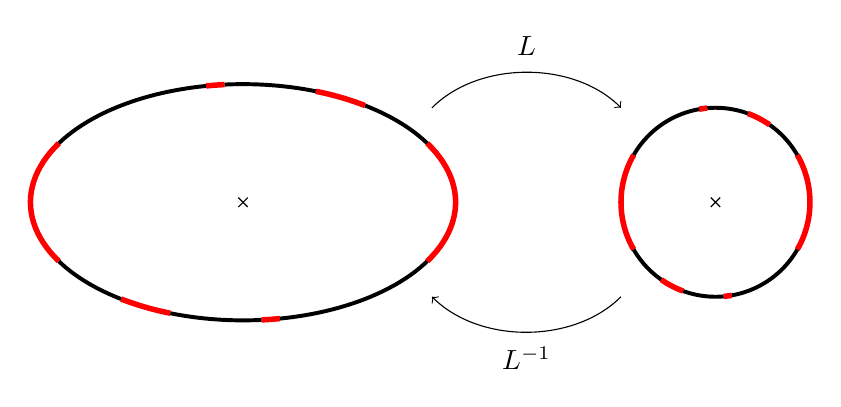
\begin{tikzpicture}[scale=0.6]
\draw (-4-0.1,-0.1) -- (-4+0.1,0.1);
\draw (-4-0.1,0.1) -- (-4+0.1,-0.1);
\draw [line width = 0.7mm,red,domain=-30:30] plot ({-4 + 4.5 * cos(\x)}, {2.5 * sin(\x)});
\draw [line width = 0.5mm,black,domain=30:55] plot ({-4 + 4.5 * cos(\x)}, {2.5 * sin(\x)});
\draw [line width = 0.7mm,red,domain=55:70] plot ({-4 + 4.5 * cos(\x)}, {2.5 * sin(\x)});
\draw [line width = 0.5mm,black,domain=70:95] plot ({-4 + 4.5 * cos(\x)}, {2.5 * sin(\x)});
\draw [line width = 0.7mm,red,domain=95:100] plot ({-4 + 4.5 * cos(\x)}, {2.5 * sin(\x)});
\draw [line width = 0.5mm,black,domain=100:150] plot ({-4 + 4.5 * cos(\x)}, {2.5 * sin(\x)});
\draw [line width = 0.7mm,red,domain=150:210] plot ({-4 + 4.5 * cos(\x)}, {2.5 * sin(\x)});
\draw [line width = 0.5mm,black,domain=210:235] plot ({-4 + 4.5 * cos(\x)}, {2.5 * sin(\x)});
\draw [line width = 0.7mm,red,domain=235:250] plot ({-4 + 4.5 * cos(\x)}, {2.5 * sin(\x)});
\draw [line width = 0.5mm,black,domain=250:275] plot ({-4 + 4.5 * cos(\x)}, {2.5 * sin(\x)});
\draw [line width = 0.7mm,red,domain=275:280] plot ({-4 + 4.5 * cos(\x)}, {2.5 * sin(\x)});
\draw [line width = 0.5mm,black,domain=280:330] plot ({-4 + 4.5 * cos(\x)}, {2.5 * sin(\x)});

\draw (5.9,-0.1) -- (6.1,0.1);
\draw (5.9,0.1) -- (6.1,-0.1);
\draw [line width = 0.7mm,red,domain=-30:30] plot ({6 + 2 * cos(\x)}, {2 * sin(\x)});
\draw [line width = 0.5mm,black,domain=30:55] plot ({6 + 2 * cos(\x)}, {2 * sin(\x)});
\draw [line width = 0.7mm,red,domain=55:70] plot ({6 + 2 * cos(\x)}, {2 * sin(\x)});
\draw [line width = 0.5mm,black,domain=70:95] plot ({6 + 2 * cos(\x)}, {2 * sin(\x)});
\draw [line width = 0.7mm,red,domain=95:100] plot ({6 + 2 * cos(\x)}, {2 * sin(\x)});
\draw [line width = 0.5mm,black,domain=100:150] plot ({6 + 2 * cos(\x)}, {2 * sin(\x)});
\draw [line width = 0.7mm,red,domain=150:210] plot ({6 + 2 * cos(\x)}, {2 * sin(\x)});
\draw [line width = 0.5mm,black,domain=210:235] plot ({6 + 2 * cos(\x)}, {2 * sin(\x)});
\draw [line width = 0.7mm,red,domain=235:250] plot ({6 + 2 * cos(\x)}, {2 * sin(\x)});
\draw [line width = 0.5mm,black,domain=250:275] plot ({6 + 2 * cos(\x)}, {2 * sin(\x)});
\draw [line width = 0.7mm,red,domain=275:280] plot ({6 + 2 * cos(\x)}, {2 * sin(\x)});
\draw [line width = 0.5mm,black,domain=280:330] plot ({6 + 2 * cos(\x)}, {2 * sin(\x)});
\draw[->] (0,2) .. controls (1,3) and (3,3)
.. (4,2);
\draw[->] (4,-2) .. controls (3,-3) and (1,-3)
.. (0,-2); 
\draw (2,3.3) node {$L$};
\draw (2,-3.3) node {$L^{-1}$};
\end{tikzpicture}
\end{center}


Thus, we consider now the sphere $\sphere$ with a given a subset $X_{\epsilon} \in \sphere$ that might violate our contractivity constraint. We consider the following property of linear switched systems.

\begin{property}\label{property:convpres}
The dynamics given in \eqref{eq:switchedSystem} is convexity-preserving, meaning that for any set of points $X \subset \R^n$ we have:
$$ f(\conv({X}))\subset \conv(f(X)). $$
\end{property}


This leads us to look for the largest ball in $\convhull (S \setminus X_{\epsilon})$. Indeed, by Property~\ref{property:convpres}, we know that the image by our system $f$ of this ball will be in $\convhull (S \setminus X_{\epsilon})$, i.e., the ball will expand in $\ball$ with ratio at most $\frac{1}{\delta}$, where $\delta$ denotes the radius of that largest ball. 

We investigate then the case for which the largest ball included $\convhull (S \setminus X_{\epsilon})$ has the smallest radius, which will maximize our upper bound on the growth of rate of the ball considered, and thus will give us an upper bound on the JSR equal to $\frac{\gamma^{*}}{\delta}$. Minimizing $\delta$ will then give us the worst case set for a given measure $\epsilon$ of points authorized to violate our constraint. This worst case will happen when the set of violating points on $\sphere$ is a spherical cap (see \ref{thm:mainSphericalCap} in the appendix). Let us define this notion.


\begin{definition}
We define the \emph{spherical cap} on $\sphere$ for a given hyperplane $c^Tx = k$ as:
\begin{equation*}\calC_{c,k} := \{x \in \sphere : c^Tx >k\}.
\end{equation*}
\end{definition}

\begin{center}
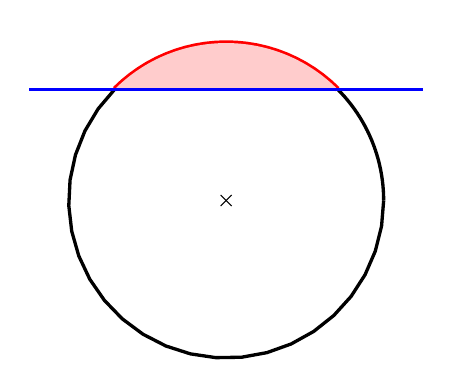
\begin{tikzpicture}
\draw (-0.07,-0.07) -- (0.07,0.07);
\draw (-0.07,0.07) -- (0.07,-0.07);
\draw [black,very thick,domain=0:45] plot ({2*cos(\x)}, {2*sin(\x)});
\draw [line width = 0.7mm,red,domain=45:135] plot ({2*cos(\x)}, {2*sin(\x)});
\draw [black,very thick,domain=135:360] plot ({2*cos(\x)}, {2*sin(\x)});
\fill[fill=red!20] (1.414,1.414) arc [start angle=45, end angle=135, radius=2] -- cycle;
\draw[blue, very thick] (-2.5,1.414) -- (2.5,1.414);
\end{tikzpicture}
\end{center}

For a given spherical cap of area measure $\epsilon$, we can compute a closed form expression of the radius of the corresponding largest ball. We denote by $\alpha$ the function that associates to each $\epsilon \in [0,1]$ the value of this radius. We have an expression for $\alpha$ given by the following lemma (see the appendix for details of its proof).

\begin{lemma}\label{lemma:eps}
Let $\epsilon \in (0, \frac{1}{2})$ and $\alpha: (0,1) \to \R_{\geq 0}$ be defined by:
\begin{equation}\label{eqn:ballinc}
\alpha(\epsilon) := \inf_{X \in \calX_\epsilon} \sup\{r: r\ball \subset \convhull(\sphere \setminus X)\},
\end{equation}
where $\calX_{\epsilon} = \{X \subset \sphere: \sigma^{n-1}(X) \leq \epsilon\}$. Then, $\alpha(\epsilon)$ is given by the formula:
\begin{equation}\label{eqn:alphaEpsilon}
\alpha(\epsilon) = \sqrt{1- I^{-1}\left(2\epsilon; \frac{n-1}{2}, \frac{1}{2}\right)}, \end{equation}
where $I$ is the regularized incomplete beta function.
\end{lemma}

Since $f$ is homogeneous, we will have in fact $X_{\epsilon}$ union of two spherical caps, each of measure $\frac{\epsilon}{2}$. We illustrate the problem when $X_{\epsilon}$ is a this form.

\begin{center}
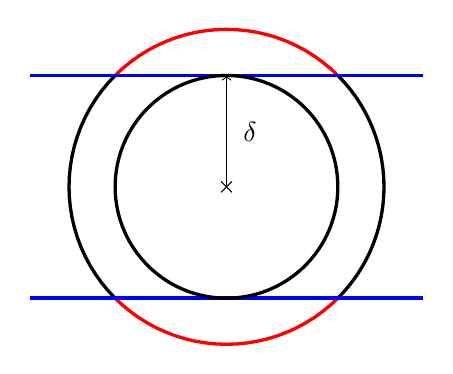
\begin{tikzpicture}
\draw (-0.07,-0.07) -- (0.07,0.07);
\draw (-0.07,0.07) -- (0.07,-0.07);
\draw [black,very thick,domain=0:45] plot ({2*cos(\x)}, {2*sin(\x)});
\draw [red,very thick,domain=45:135] plot ({2*cos(\x)}, {2*sin(\x)});
\draw [black,very thick,domain=135:225] plot ({2*cos(\x)}, {2*sin(\x)});
\draw [red,very thick,domain=225:315] plot ({2*cos(\x)}, {2*sin(\x)});
\draw [black,very thick,domain=315:360] plot ({2*cos(\x)}, {2*sin(\x)});
\draw[line width = 0.5mm,blue] (-2.5,1.414) -- (2.5,1.414);
\draw[line width = 0.5mm,blue] (-2.5,-1.414) -- (2.5,-1.414);
\draw[->] (0,0) -- (0,1.414);
\draw (0.3,0.7) node {$\delta$};
\draw [black,very thick] (0,0) circle [radius = 1.414cm];
\end{tikzpicture}
\end{center}


Let us now formally prove the transformation of our initial problem to the geometric one. By exploiting Property \ref{property:convpres} above, we first show in Lemma \ref{lemma:epsilon1} how one can compute an upper bound on the JSR when the ``almost invariant" set is the unit sphere $\sphere$.

\begin{lemma}\label{lemma:epsilon1}
Let $\epsilon \in (0, 1)$ and $\gamma \in \R_{> 0}$. Consider the set of matrices $\calM$ and $A \in \calM^l$ satisfying:
\begin{equation}\label{eqn:contraction}
(A_{j_l} A_{j_{l-1}} \dots A_{j_1} x)^T (A_{j_l} A_{j_{l-1}} \dots A_{j_1} x) \leq \gamma^{2l} x^Tx, \quad \forall\, x \in \sphere \setminus \sphere', \forall\,(j_1, \dots, j_l) \in M^l,
\end{equation}
where $\sphere' \subset \sphere$ and $\sigma^{n-1}(\sphere') \leq \epsilon$, then we have:
\begin{equation*}
\rho(\calM) \leq \frac{\gamma}{\sqrt[l]{\alpha(\epsilon)}}}
\end{equation*}
where $\alpha(\epsilon)$ is given in \eqref{eqn:alphaEpsilon}.
\end{lemma}
%
\begin{proof}
Note that, \eqref{eqn:contraction} implies that:
$(A_{j_l} A_{j_{l-1}} \dots A_{j_1}) (\sphere \setminus \sphere') \subset \gamma^l \ball.$
Using Property \ref{property:convpres} this also implies:
$$A_{j_l} A_{j_{l-1}} \dots A_{j_1} \left( \convhull(\sphere \setminus \sphere') \right) \subset \convhull \left( A_{j_l} A_{j_{l-1}} \dots A_{j_1}(\sphere \setminus \sphere') \right) \subset \gamma^l \ball .$$
Then, by Lemma \ref{lemma:eps} in Appendix \ref{app:eps}, we have:
$$A_{j_l} A_{j_{l-1}} \dots A_{j_1} \left( \alpha(\epsilon) \ball \right) \subset A_{j_l} A_{j_{l-1}} \dots A_{j_1} \left( \convhull (\sphere \setminus \sphere') \right) \subset \gamma^l\ball, \quad  \forall\, (j_1, \dots, j_l) \in M^l,$$
by definition of $\alpha(\epsilon)$ given in \eqref{eqn:ballinc}. Therefore, we get:
$$\alpha(\epsilon) \left( A_{j_l} A_{j_{l-1}} \dots A_{j_1} (\ball) \right) \subset \gamma^l\ball,$$
which implies that $\rho(\calM^l) \leq \frac{\gamma^l}{\alpha(\epsilon)}$ and hence $\rho(\calM) \leq \frac{\gamma}{\sqrt[l]{\alpha(\epsilon)}}$.
\end{proof}










%\begin{lemma}\label{lemma:epsilon1}Let $\epsilon \in (0, 1)$ and $\gamma \in \R_{> 0}$. Consider the set of matrices $\calM$ and $A \in \calM$ satisfying:
%\begin{equation}\label{eqn:contraction}(A_jx)^T(A_jx) \leq \gamma^2 x^Tx, \quad \forall\, x \in \sphere \setminus \sphere', \forall\,j \in, M,\end{equation}
%where $\sphere' \subset \sphere$ and $\sigma^{n-1}(\sphere') \leq \epsilon$, then we have:
%\begin{equation*}
%\rho(\calM) \leq \frac{\gamma}{\alpha(\epsilon)}
%\end{equation*}
%where $\alpha(\epsilon)$ is given in \eqref{eqn:alphaEpsilon}.
%\end{lemma}
%
%\begin{proof}Note that, \eqref{eqn:contraction} implies that:
%$A_j (\sphere \setminus \sphere') \subset \gamma \ball.$
%Using Property \ref{property:convpres} this also implies:
%$$A_j \convhull(\sphere \setminus \sphere') \subset \convhull(A_j(\sphere \setminus \sphere')) \subset \gamma \ball .$$
%Then, by Lemma \ref{lemma:eps} in Appendix \ref{app:eps}, we have:
%$$A_j (\alpha(\epsilon) \ball) \subset A_j (\convhull (\sphere \setminus \sphere')) \subset \gamma\ball, \quad  \forall\, j \in M,$$
%by definition of $\alpha(\epsilon)$ given in \eqref{eqn:ballinc}. Therefore, we get:
%$$\alpha(\epsilon) A_j (\ball) \subset \gamma\ball,$$
%which implies that $\rho(\calM) \leq \frac{\gamma}{\alpha(\epsilon)}.$
%\end{proof}

We now know how to compute an upper bound on the JSR when the ``almost invariant" ellipsoid is $\sphere$. Thanks to Property \ref{rem:scaling}, if this is not the case, we can simply perform a change of coordinates mapping this ellipsoid to $\sphere$ and compute the JSR in the new coordinates system instead. To do this, in the next theorem, we bound the measure of violating constraints on $\sphere$ after the change of coordinates, in terms of the measure of the violated constraints on $\sphere \times M^l$ in the original coordinates.
%This is thanks to the homogeneity of the dynamics stated in Property \ref{property:homogeneity}.

\begin{theorem}\label{thm:mainTheorem01}
Let $\gamma \in \R_{> 0}$. Consider a set of matrices $\calM$, and a matrix $P \succ 0$ satisfying:
\begin{equation}\label{eqn:P0}
(A_{j_l} A_{j_{l-1}} \dots A_{j_1} x)^T P(A_{j_l} A_{j_{l-1}} \dots A_{j_1} x) \leq \gamma^{2l} x^T P x,\,\, \forall\, (x, j_1, \dotsc, j_l) \in Z_l \setminus V,
\end{equation}
for some $V \subset Z_l$ where $\mu_l(V) \leq \epsilon$. Then
%Then, by defining $L$ as in \eqref{choleski} and $\bar{A_j}=  L^{-1}A_jL$, one also has:
%\begin{equation*}\label{eqn:thm01-2}(\bar{A_j} x)^T(\bar{A_j} x) \leq {\gamma}^2x^Tx,\,\, \forall\, x \in \sphere \setminus \sphere', \forall\, j \in M,\end{equation*}
\begin{equation*}\label{eqn:thm01-2}
(A_{j_l} A_{j_{l-1}} \dots A_{j_1} x)^T (A_{j_l} A_{j_{l-1}} \dots A_{j_1} x) \leq \gamma^{2l} x^T x,\,\, \forall\, x \in \sphere \setminus \sphere', \forall\, (j_1,\dots,j_l) \in M^l,
\end{equation*}
for some $\sphere' \subset \sphere$ such that: $\sigma(\sphere') \leq m^l \epsilon \kappa(P),$
where $$\kappa(P) = \sqrt{\frac{\lambda_{\max}(P)^n}{\det(P)}}.$$
\end{theorem}

\begin{proof}
Let $V_{\sphere} = \pi_{\sphere}(V)$. We know that $\Sigma_{M^l}$ is the disjoint union of its $2^{m^l}$ elements $\{\calM^l_i, i \in \{1,2, \dots, 2^{m^l} \} \}$. Then $V$ can be written as the disjoint union $V = \sqcup_{1 \leq i \leq 2^{m^l}} (\calS_i, \calM^l_i)$ where $\calS_i \in \Sigma_{\sphere}$. We notice that 
$V_{\sphere} = \sqcup_{1 \leq i \leq 2^{m^l}} \calS_i$, 
and
\begin{equation*}
\sigma^{n-1} (V_{\sphere}) = \sum_{1 \leq i \leq 2^{m^l}} \sigma^{n-1} (\calS_i).
\end{equation*}
We have 
\begin{eqnarray*}
\mu_l(V) &=& \mu_l \left( \sqcup_{1 \leq i \leq 2^{m^l}} (\calS_i, \calM^l_i) \right) = \sum_{1 \leq i \leq 2^{m^l}} \mu_l(\calS_i, \calM^l_i) \\
 &=& \sum_{1 \leq i \leq 2^{m^l}} \sigma^{n-1} \otimes \mu_{M^l} (\calS_i, \calM^l_i) \\
 & = &\sum_{1 \leq i \leq 2^{m^l}} \sigma^{n-1}(\calS_i) \mu_{M^l} (\calM^l_i).
\end{eqnarray*}
Note that we have $\min_{(j_1,\dots,j_l) \in M^l} \mu_{M^l}(\{j_1,\dots,j_l\}) = \frac{1}{m^l}.$ Then since $ \forall \ i$, $\mu_{M^l}(\calM^l_i) \geq \min_{(j_1,\dots,j_l) \in M^l} \mu_{M^l}(\{j_1,\dots,j_l\}) = \frac{1}{m^l}$, we get:
\begin{equation}
\sigma^{n-1}(V_{\sphere}) \leq \frac{\mu_l(V)}{\frac{1}{m^l}} \leq m^l \epsilon.
\end{equation}
This means that 
\begin{equation}\label{eqn:P2}
(A_{j_l} A_{j_{l-1}} \dots A_{j_1} x)^T P (A_{j_l} A_{j_{l-1}} \dots A_{j_1} x) \leq \gamma^{2l} x^T P x,\,\, \forall\, x \in \sphere \setminus V_\sphere, \,\forall\, (j_1,\dots,j_l) \in M^l,
\end{equation}
where $\sigma^{n-1}(V_\sphere) \leq m^l \epsilon.$

We then perform the change of coordinates defined by $L^{-1} \in \calL(\R^n)$ which maps $\sphere$ to $E_P$, defined as in \eqref{choleski}. By defining $\bar{A_{j_i}}=  L^{-1} A_{j_i} L$, one has:
\begin{equation*}\label{eqn:thm01-2}
(\bar{A_{j_l}} \bar{A_{j_{l-1}}} \dots \bar{A_{j_1}} x)^T (\bar{A_{j_l}} \bar{A_{j_{l-1}}} \dots \bar{A_{j_1}} x) \leq {\gamma}^{2l} x^T x,\,\, \forall\, x \in \sphere \setminus \sphere', \forall\, (j_1,\dots,j_l) \in M^l.
\end{equation*}
We can then rewrite
\eqref{eqn:P2} in this new coordinates system as in: 
\begin{equation}
(\bar{A_{j_l}} \bar{A_{j_{l-1}}} \dots \bar{A_{j_1}} x)^T (\bar{A_{j_l}} \bar{A_{j_{l-1}}} \dots \bar{A_{j_1}} x) \leq {\gamma}^{2l} x^T x,\,\, \forall\, x \in E_P\setminus L^{-1}(V_\sphere), \,\forall\, (j_1,\dots,j_l) \in M^l.
\end{equation}

Due to the  the homogeneity of the dynamics described in Property \ref{property:homogeneity}, this implies:
\begin{equation}\label{eqn:P}
(\bar{A_{j_l}} \bar{A_{j_{l-1}}} \dots \bar{A_{j_1}} x) \leq \gamma^{2l} x^T x,\,\, \forall\, x \in \sphere \setminus \proj_\sphere(L^{-1}(V_\sphere)), \,\forall\, (j_1,\dots,j_l) \in M^l.
\end{equation}
Thanks to the Property~\ref{rem:scaling}, we even have:
\begin{equation}\label{eqn:P1}
(A_{j_l} A_{j_{l-1}} \dots A_{j_1} x) \leq \gamma^{2l} x^T x,\,\, \forall\, x \in \sphere \setminus \proj_\sphere(L^{-1}(V_\sphere)), \,\forall\, (j_1,\dots,j_l) \in M^l.
\end{equation}
%We now show how to relate $\sigma^{n-1}({V_\sphere})$ to $\sigma^{n-1}(\proj_\sphere(L^{-1}(V_\sphere)))$. Note that, since $L \in \calL({\R^n})$ by Remark \ref{rem:mappingMeasures} we have:
%\begin{equation}\label{eqn:det}\sigma_P(L^{-1}(V_\sphere)) = |\det(L^{-1})| \sigma^{n-1}(V_\sphere).\end{equation}

We now show how to relate $\sigma^{n-1}(V_\sphere)$ to $\sigma^{n-1}(\proj_\sphere(L^{-1}(V_\sphere)))$. Consider $\sphere^{V_{\sphere}}$, the sector of $\ball$ defined by $V_{\sphere}$. We denote $C:= L^{-1}(\sphere^{V_{\sphere}})$ and $V':=\proj_\sphere(L^{-1}(V_\sphere))$. We have $\proj_{\sphere}(C) = V'$ and $\sphere^{V'} \subset \calH_{1/ \lambda_{\min}(L^{-1})}(C),$
where $\calH$ is the homothety of ratio $1/ \lambda_{\min}(L^{-1})$. This leads to:
$$\sigma^{n-1}(V') = \lambda(\sphere^{V'}) \leq \lambda (\calH_{1/ \lambda_{\min}(L^{-1})}(C)).$$ Then, the following holds: \begin{eqnarray}\nonumber\sigma^{n-1}(V') &\leq& \frac{1}{\lambda_{\min}(L^{-1})^n}\lambda(C) \\
\nonumber &\leq&\frac{1}{\lambda_{\min}(L^{-1})^n} \lambda( L^{-1}(\sphere^{V_{\sphere}}))\\ 
\label{eqn:lt} &=&\frac{|\det(L^{-1})|}{\lambda_{\min}(L^{-1})^n}\lambda(\sphere^{V_\sphere}),\\
 \label{eqn:map1} &=&\sqrt{\frac{\lambda_{\max}(P)^n}{\det(P)}}\sigma^{n-1}(V_\sphere)
\end{eqnarray}
where \eqref{eqn:lt} follows from the fact that
$$ \lambda(Q(X)) = |\det(Q)| \lambda(X),$$
for any set $X \subset \R^n$ and $Q \in \calL(\R^n)$ (see e.g. \cite{rudin}).
Putting together \eqref{eqn:P2}, \eqref{eqn:P1}, and \eqref{eqn:map1} we get the statement of the theorem where $\sphere' = \proj_\sphere(L^{-1}(V_\sphere)).$
%Then, if we let $E':=L^{-1} V_\sphere$, where $L$ is the linear transformation mapping $E_P$ to $\sphere$, we get: $$\sigma_P(E') = \sigma^{n-1}(V_\sphere), and the result of the theorem follows.
\end{proof}

\begin{remark}
We are now ready to prove our main theorem by putting together all the above pieces. For a given level of confidence $\beta,$ we prove that the upper bound $\gamma^{*}(\omega_N)$, which is valid solely on finitely many observations, is in fact a true upper bound, at the price of increasing it by the factor $\frac{1}{\delta(\beta, \omega_N)}$. Moreover, as expected, this factor gets smaller as we increase $N$ and decrease $\beta$.
\end{remark}
%
%
%\begin{proposition}\label{thm:mainTheorem01}Let $\gamma \in \R_{> 0}$. Consider a set of matrices $A \in \calM$, and a matrix $P \succ 0$ satisfying:
%\begin{equation}\label{eqn:P0}(A_j x)^TP(A_j x) \leq {\gamma}^2x^TPx,\,\, \forall\, (x, j) \in Z \setminus V,\end{equation}
%for some $V \subset Z$ where $\mu(V) \leq \epsilon$. Then, by defining $L$ as in \eqref{choleski} and $\bar{A_j}=  L^{-1}A_jL$, one also has:
%\begin{equation*}\label{eqn:thm01-2}(\bar{A_j} x)^T(\bar{A_j} x) \leq {\gamma}^2x^Tx,\,\, \forall\, x \in \sphere \setminus \sphere', \forall\, j \in M,\end{equation*}
%for some $\sphere' \subset \sphere$ such that: $\sigma(\sphere') \leq 1 - (1-\epsilon) \kappa(P),$
%where $$\kappa(P) = \sqrt{\frac{\lambda_{\min}(P)^n}{\det(P)}}.$$
%\end{proposition}
%
%\begin{proof}Let $\bar{V}_{\sphere} = \pi_{\sphere}(Z \setminus V)$. We know that $\Sigma_M$ is the disjoint union of its $2^m$ elements $\{\calM_i, i \in \{1,2, \ldots 2^m\} \}$. Then $Z \setminus V$ can be written as the disjoint union $Z \setminus V= \sqcup_{1 \leq i \leq 2^m} (\calS_i, \calM_i)$ where $\calS_i \in \Sigma_{\sphere}$. We notice that 
%$\bar{V}_{\sphere} = \sqcup_{1 \leq i \leq 2^m} \calS_i$, 
%and
%\begin{equation*}
%\sigma^{n-1} (\bar{V}_{\sphere}) = \sum_{1 \leq i \leq 2^m} \sigma^{n-1} (\calS_i).
%\end{equation*}
%We have 
%\begin{eqnarray*}
%\mu(Z \setminus V) &=& \mu(\sqcup_{1 \leq i \leq 2^m} (\calS_i, \calM_i)) = \sum_{1 \leq i \leq 2^m} \mu(\calS_i, \calM_i) \\
% &=& \sum_{1 \leq i \leq 2^m} \sigma^{n-1} \otimes \mu_M (\calS_i, \calM_i) \\
% & = &\sum_{1 \leq i \leq 2^m} \sigma^{n-1}(\calS_i) \mu_M (\calM_i).
%\end{eqnarray*}
%Note that we have $\mu_M (\calM_i) \leq 1$, and we get:
%\begin{equation}
%\mu(Z \setminus V) \leq \sigma^{n-1}(\bar{V}_\sphere),
%\end{equation}
%and therefore
%\begin{equation}
%\sigma^{n-1}(\bar{V}_{\sphere}) \geq \mu(Z \setminus V) \geq 1-\epsilon.
%\end{equation}
%This means that 
%\begin{equation}\label{eqn:P2}(A_j x)^TP(A_j x) \leq {\gamma}^2x^TPx,\,\, \forall\, x \in \sphere \setminus V_\sphere, \,\forall\, m \in M,\end{equation}
%where $\sigma^{n-1}(S \setminus V_\sphere) \geq 1 - \epsilon$.
%By similar arguments to the previous theorem we get:
%\begin{equation*}\label{eqn:thm01-2}(\bar{A_j} x)^T(\bar{A_j} x) \leq {\gamma}^2x^Tx,\,\, \forall\, x \in \sphere \setminus \sphere', \forall\, j \in M,\end{equation*}
%for some $\sphere' \subset \sphere$ such that: $\sigma(\sphere' \setminus \sphere) \geq (1 - \epsilon) \kappa_{\min}(P),$
%where $$\kappa_{\min}(P) = \sqrt{\frac{\lambda_{\min}(P)^n}{\det(P)}},$$
%which means $$\sigma(\sphere') \leq 1 - (1 - \epsilon) \kappa_{\min}(P).$$
%\end{proof}
%
%\begin{theorem}\label{thm:mainTheorem1}Let $\epsilon \in (0,1)$ and $\gamma \in \R_{> 0}$. Consider a set of matrices $A \in \calM$, and an ellipsoid $E_P$ satisfying:
%\begin{equation}\label{eqn:ellipsoid}(A_j x)^TP(A_j x) \leq \gamma^2x^TPx,\,\, \forall\, x \in E_P \setminus E', \forall\, j \in M, \end{equation}
%for some $E' \subset E$ and $\sigma_P(E') \leq \epsilon$, then we can compute $\bar{\alpha}(\epsilon) > 0$ such that we have:
%\begin{equation}\label{eqn:contractionEllipsoid}A_j \tilde{E}_P \subset \frac{\gamma}{\bar{\alpha}(\epsilon)}\tilde{E}_P, \forall\, j \in M.
%\end{equation}
%\end{theorem}
%where, $\lim_{\epsilon \to 0} \bar{\alpha}(\epsilon) = 1$.


%\begin{proof} We first rewrite the inequality in \eqref{eqn:ellipsoid} under the linear transformation $L$ which maps the ellipsoid $E_P$ to $\sphere$ as follows:
%\begin{equation}(\bar{A}_j x)^T(\bar{A}_j x) \leq \gamma^2x^Tx,\,\, \forall\, x \in \sphere \setminus \sphere', \forall\, j \in M, \end{equation}
%
%
%Due to Property \ref{property:homogeneity}, the inequality in \eqref{eqn:ellipsoid} implies
%\begin{equation}(A_j x)^TP(A_j x) \leq \gamma^2x^TPx,\,\, \forall\, x \in \sphere \setminus \proj_\sphere(E'), \forall\, j \in M, \end{equation}
%
%
%
%Let $V_\sphere:=\proj_\sphere(V)$. Let us consider $S^{V_{\sphere}}$ the sector of $\ball$ defined by $V_{\sphere}$. We denote $C:= L(S^{V_{\sphere}})$. We have $\proj_{\sphere}(C) = V'$ and $S^{V'} \subset \calH_{1/ \lambda_{\min}(L^{-1})}(C)$.  We have then 
%$$\sigma^{n-1}(V') = \lambda(S^{V'}) \leq \lambda (\calH_{1/ \lambda_{\min}(L^{-1})}(C)),$$ which means: $$\sigma^{n-1}(V') \leq \frac{1}{\lambda_{\min}(L^{-1})^n} \lambda(C).$$ Using Remark \ref{rem:mappingMeasures}, we have the result of the theorem.
%\end{proof}

%
%\begin{theorem}\label{thm:mainTheorem}Consider an $n$-dimensional switching system as in \eqref{eq:switchedSystem}. For any given $\beta \in (0,1]$ and a uniform random sampling $\omega_N \subset Z$, with $N \geq \frac{n(n+1)}{2}+1$, and let $\gamma^*(\omega_N) $ be the optimal solution to \eqref{eqn:campiOpt01}. Then, we can compute $\delta(\beta, \omega_N)$, such that with probability at least $\beta$ we have:
%$$\rho \leq \frac{\gamma^*(\omega_N)}{\delta(\beta, \omega_N)},$$
%where $\lim_{N \to \infty}\delta(\beta, \omega_N) = 1$.
%\end{theorem}
%
%\begin{proof}
%Note that, by definition of $\gamma^*(\omega_N)$ we have:
%\begin{equation*} (A_j x)^TP(A_j x) \leq {\gamma^*}^2 x^TPx, \quad \forall\, (x, j)  \in \omega_N \end{equation*}
%for some $P \succ 0$. 
%Note that the inequality \eqref{eqn:violation} in Theorem \ref{mainTheorem0} can be also written as:
%\begin{equation}\label{eqn:violation2}\mathbb{P}^N\left\{ \mu(V(\omega_N)) \leq \epsilon \right\} \geq I(\epsilon; d+1, N-d),\end{equation}
%where $I(\ell;a,b)$ is the regularized in complete beta function. Then, for all $\epsilon \in (0,1)$ satisfying:
%\begin{equation}\label{eqn:eps}\epsilon \leq 1- I^{-1}(\beta, d+1, N-d),\end{equation} we have $\mathbb{P}^N\left\{ \mu(V(\omega_N)) \leq \epsilon \right\} \geq \beta$.
%Then, by Theorem \ref{thm:mainTheorem01} for all $\epsilon$ satisfying \eqref{eqn:eps}, with probability at least $\beta$ the following holds:
%\begin{equation*} (A_jx)^TP(A_jx) \leq  {\gamma^*}^2 x^TPx, \quad \forall (x, j) \in Z \setminus V,\end{equation*}
%for some $V \subset Z$, where $\mu(Z) \leq \epsilon$. By Theorem \ref{thm:mainTheorem01}, this implies that with probability at least $\beta$ the following also holds:
%\begin{equation} \label{eqn:mainthm1}(A_jx)^TP(A_jx) \leq  {\gamma^*}^2 x^TPx, \quad \forall x \in E_P \setminus E', \forall\, j \in M,\end{equation}
%for some $E'$ where $\sigma_P(E') \leq m \epsilon$. The inequality in \eqref{eqn:mainthm1} can be rewritten as:
%\begin{equation}\label{eqn:mainthm2}\frac{A_j}{\gamma^*}(E_P \setminus E') \subset \tilde{E}_P,\quad \forall j \in M.
%\end{equation}
%Note that, $E_P \subset \tilde{E}_P$. Using this fact, along with \eqref{eqn:mainthm2} and Property \ref{property:convpres}, we get:
%\begin{eqnarray*}\frac{A_j}{\gamma^*}\convhull(E_P \setminus E') &\subset& \convhull \left(\frac{A_j}{\gamma^*} \left(E_P \setminus E'\right) \right)\\ &\subset& \convhull\left(\frac{A_j}{\gamma^*}\tilde{E}_P\right), \,\, \forall\, j \in M.
%\end{eqnarray*}
%
%
%
%$$\frac{\calM}{\gamma^*} \conv(E_P \setminus E') \subset \convhull(E_P \setminus E'),$$
%for some $E' \subset E_P$, where $\sigma_P(E') \leq \epsilon$.
%Then, due to Theorem \ref{thm:mainTheorem0} we also have \eqref{eqn:contraction}, meaning:
%$$\left(\frac{\cM}{\delta \gamma^*}\right) \convhull (E_P \setminus X_P) \subset \convhull (E_P\setminus X_P).$$
%Then, $\delta\gamma^*$ is an upper bound on $\rho,$ with probability at least~$\beta$. 
%\end{proof}


%Note that if $P$ is a solution of \eqref{eqn:campiOpt0}, due to Property \ref{property:homogeneity}, then so is $\alpha P$ for any $\alpha \in \R_{> 0}.$ Therefore, the constraint $P \succ 0$ can be replaced with the constraint $P \succeq I$. 
%In this section, we show that using Property \ref{property:homogeneity} and Property \ref{property:convpres}, by sampling finitely many points on a level set of a candidate CQLF, we can compute an upper bound on $\rho$. This section formalizes this discussion. Before proceeding to the main theorem, we motivate the upcoming technical discussion by stating the following theorem to which most of this section is devoted.
%
%\begin{theorem} \label{thm:mainTheorem0} Let $\epsilon \in (0,1]$, $\beta \in [0,1)$. Consider a uniform random sampling of $\sphere \times M$, denoted by $\omega_N$. Let $\gamma^*$ and $P$ be the optimal solution to:
%\begin{equation}\label{eqn:campiOpt01}
%\begin{aligned}
%& \text{min} & & \gamma \\
%& \text{s.t.} 
%&  & (A_j x)^TP(A_j x) \leq \gamma x^TPx,\,\forall (x, j) \in \omega_N \\
%& && P \succ 0. \\
%\end{aligned}
%\end{equation}
%Then for all $Z_P$ with $\sigma_P(Z_P)\leq \epsilon$, we have with probability at least $\beta$:
%\begin{equation} \label{eqn:exceptEps}(A_j x)^TP(A_j x)\leq \gamma^*x^TPx,\,\forall\, x \in E_P \setminus Z_P, \forall j \in M.\end{equation}
%Moreover, we can compute $\delta(\beta, \omega_N) < \infty$  such that:
%\begin{equation}\label{eqn:contraction}E_{\delta^2P} \subset  \convhull (E_{P} \setminus Z_{P}),
%\end{equation}
%and $\lim_{N \to \infty} \delta(\beta, \omega_N) = 1.$
%\end{theorem}
%
%Once Theorem \ref{thm:mainTheorem0} is established, the main result of this section follows.
%
%\begin{theorem}[Main Theorem] \label{thm:mainTheorem} Let $\omega_N$ be a uniform sampling of $\sphere \times M$, where $N \geq \frac{n(n+1)}{2}+1$ and $\beta \in [0,1)$. We can compute $\delta(\beta, \omega_N) < \infty$ such that with probability at least $\beta$ we have $$\rho \leq \frac{\gamma^*(\omega_N)}{\delta}.$$ Moreover, $\lim_{N \to \infty} \delta(\beta, \omega_N) = 1$.
%\end{theorem}
%
%%\begin{theorem}
%%Consider a black-box switching system and $N$ samples of its dynamics as in \eqref{eq:switchedSystem}. Consider the optimal solution $(\lambda^*,P)$ which minimizes $\lambda$ in \eqref{eq:lowerbound}. For any factor $1<\delta,$ one can compute the level of confidence $\beta$ such that $\rho<\delta\cdot\lambda^*.$ 
%%% denote $\gamma(P,\epsilon)$ the largest $\gamma$ such that $\gamma^2y_i^TPy_i\leq x_i^TPx_i$ 
%%\end{theorem}
%\begin{proof}Note that, by definition of $\gamma^*$ we have:
%\begin{equation*} (A_j x)^TP(A_j x) \leq \gamma^* x^TPx, \quad \forall\, (x, j)  \in \omega_N \end{equation*}
%for some $P \succ 0$. Then, by Theorem \ref{thm:mainTheorem0} we have:
%\begin{equation*} (A_j x)^TP(A_j x) \leq \gamma^*x^TPx, \quad \forall\, x \in E_P \setminus Z_P,\, \forall j \in M, \end{equation*}
%which can be rewritten as:
%\begin{equation*}\frac{\calM}{\gamma^*}(E_P \setminus Z_P) \subseteq E_P \setminus Z_P.
%\end{equation*}
%By Property \ref{property:convpres}, this implies:
%$$\frac{\calM}{\gamma^*} \conv(E_P \setminus Z_P) \subset \convhull(E_P \setminus Z_P).$$
%Then, due to Theorem \ref{thm:mainTheorem0} we also have \eqref{eqn:contraction}, meaning:
%$$\left(\frac{\cM}{\delta \gamma^*}\right) \convhull (E_P \setminus Z_P) \subset \convhull (E_P\setminus Z_P).$$
%Then, $\delta\gamma^*$ is an upper bound on $\rho,$ with probability at least~$\beta$. 
%\end{proof}
